%%%%%%%%%%%%%%%%%%%%%%%%%%%%%%%%%%%%%%%%%%%%%%%%%%%%%%%%%%%%%%%%%%%%%%%%%%%%%%%%%%%%%%%%%
%             template.tex                                                              %
%                                                                                       %
%            Author: Sergej Lewin 10/2008                                               %
%                                                                                       %    
% !!!Man braucht noch die Datei Ueb.sty (im gleichen Ordner wie die Hauptdatei)!!!      %
%%%%%%%%%%%%%%%%%%%%%%%%%%%%%%%%%%%%%%%%%%%%%%%%%%%%%%%%%%%%%%%%%%%%%%%%%%%%%%%%%%%%%%%%%
\documentclass[a4paper,11pt]{article}             % bestimmt das Aussehen eines Dokuments
\usepackage{Ueb}                                  % vordefinierte Makros
\usepackage{enumitem}
\usepackage{tikz}
\renewcommand{\labelenumi}{(\alph{enumi})}
\renewcommand{\labelenumii}{(\roman{enumii})}

%!!!!anpassen an das Betriebssystem!!!, um Umlaute zu verwenden
\usepackage[utf8]{inputenc}                      %Linux
%\usepackage[latin1]{inputenc}                    %Windows
%\usepackage[applemac]{inputenc}                  %Mac



%Namen und Matrikelnummern anpassen
%\zweinamen{Name1}{Matrikelnummer1}{Name2}{Matrikelnummer2} %2er Gruppen
\dreinamen{Alexander Neuwirth}{439218}{Leonhard Segger}{440145}{Jonathan Sigrist}{441760} %3er Gruppe

%Briefkastennummer anpassen. z. B. \briefkasten{104}
\briefkasten{}

%Termin der Uebungsgruppe und Raum anpassen z. B. \termin{Mo. 12-14 , SR2}
\termin{Fr. 08-10, SR217}

%Blattnummer anpassen z. B. \blatt{5}
\blatt{9}

\begin{document}

\Aufgabe{31}
\begin{enumerate}
\item
\begin{enumerate}
\item $\mathcal O(1)$, da die Wurzel stets das kleinste Element ist.
\item $\mathcal O(n/2) = \mathcal O(n)$, da eines der Blätter das Maximum ist.
\item $\mathcal O(n)$, da jedes Element überprüft werden muss. Optimiert müssen keine Teilbäume durchsucht werden, deren Wurzel größer als das gesuchte Element sind, also $\mathcal O(n/2)$.
\item $\mathcal O(n)$, da man wie in (iii) nach einem Element sucht und dieses nicht finden wird.
\end{enumerate}

\item Jedes abzuspeichernde Element bekommt eine Zahl zugewiesen, welche pro Element im Heap zunimmt. Dabei wird ein max-Heap verwendet. Also $\texttt{max} = \mathcal O(1)$, $\texttt{delete} = \mathcal O(\log n)$ und $\texttt{insert} = \mathcal O(\log n)$.

\item Zuerst wird der Heap aufgebaut, danach kann jeweils das größte Element aus dem Heap entfernt werden indem es mit dem letzten Element vertauscht und nicht weiter betrachtet wird. Wenn der Heap leer ist, ist das gesammte Array sortiert. Der ursprüngliche und aufgebaute Heap seien gegeben mit:\\

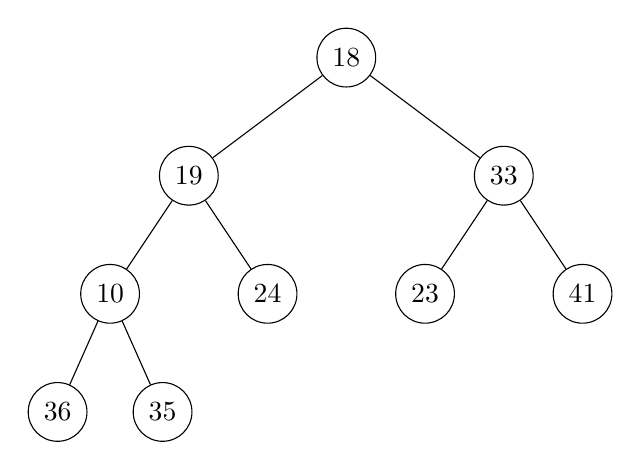
\begin{tikzpicture} [level/.style={sibling distance=40mm/#1}]
\node [circle,draw] (a) {$18$}
  child {node [circle,draw] (b) {$19$}
    child {node [circle,draw] (d) {$10$}
      child {node [circle,draw] (h) {$36$}
      }
      child {node [circle,draw] (i) {$35$}
      }
    }
    child {node [circle,draw] (e) {$24$}
    }
  }
  child {node [circle,draw] (c) {$33$}
    child {node [circle,draw] (f) {$23$}
    }
    child {node [circle,draw] (g) {$41$}
    }
  };
\end{tikzpicture}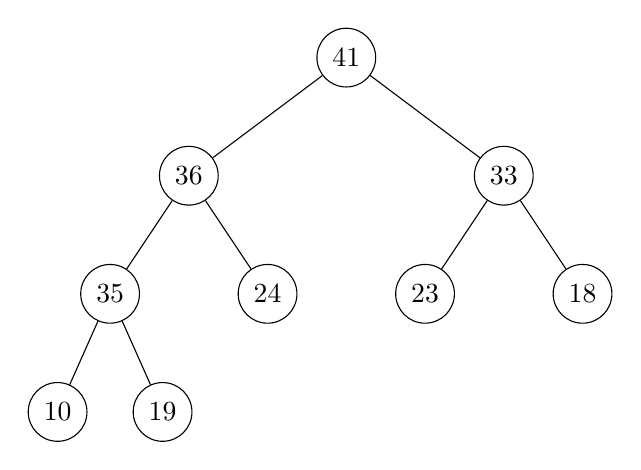
\begin{tikzpicture} [level/.style={sibling distance=40mm/#1}]
\node [circle,draw] (a) {$41$}
  child {node [circle,draw] (b) {$36$}
    child {node [circle,draw] (d) {$35$}
      child {node [circle,draw] (h) {$10$}
      }
      child {node [circle,draw] (i) {$19$}
      }
    }
    child {node [circle,draw] (e) {$24$}
    }
  }
  child {node [circle,draw] (c) {$33$}
    child {node [circle,draw] (f) {$23$}
    }
    child {node [circle,draw] (g) {$18$}
    }
  };
\end{tikzpicture}
\begin{equation*}
\begin{array}{ccccccccc}
18 & 19 & 33 & 10 & 24 & 23 & 41 & 36 & 35\\
\hline
18 & 19 & 33 & 36 & 24 & 23 & 41 & 10 & 35\\
18 & 19 & 41 & 36 & 24 & 23 & 33 & 10 & 35\\
18 & 36 & 41 & 19 & 24 & 23 & 33 & 10 & 35\\
18 & 36 & 41 & 35 & 24 & 23 & 33 & 10 & 19\\
41 & 36 & 18 & 35 & 24 & 23 & 33 & 10 & 19\\
41 & 36 & 33 & 35 & 24 & 23 & 18 & 10 & 19\\
\hline
19 & 36 & 33 & 35 & 24 & 23 & 18 & 10 & \textit{41}\\
36 & 19 & 33 & 35 & 24 & 23 & 18 & 10 & \textit{41}\\
36 & 35 & 33 & 19 & 24 & 23 & 18 & 10 & \textit{41}\\
10 & 35 & 33 & 19 & 24 & 23 & 18 & \textit{36} & \textit{41}\\
35 & 10 & 33 & 19 & 24 & 23 & 18 & \textit{36} & \textit{41}\\
35 & 24 & 33 & 19 & 10 & 23 & 18 & \textit{36} & \textit{41}\\
18 & 24 & 33 & 19 & 10 & 23 & \textit{35} & \textit{36} & \textit{41}\\
33 & 24 & 18 & 19 & 10 & 23 & \textit{35} & \textit{36} & \textit{41}\\
33 & 24 & 23 & 19 & 10 & 18 & \textit{35} & \textit{36} & \textit{41}\\
18 & 24 & 23 & 19 & 10 & \textit{33} & \textit{35} & \textit{36} & \textit{41}\\
24 & 18 & 23 & 19 & 10 & \textit{33} & \textit{35} & \textit{36} & \textit{41}\\
24 & 19 & 23 & 18 & 10 & \textit{33} & \textit{35} & \textit{36} & \textit{41}\\
10 & 19 & 23 & 18 & \textit{24} & \textit{33} & \textit{35} & \textit{36} & \textit{41}\\
23 & 19 & 10 & 18 & \textit{24} & \textit{33} & \textit{35} & \textit{36} & \textit{41}\\
18 & 19 & 10 & \textit{23} & \textit{24} & \textit{33} & \textit{35} & \textit{36} & \textit{41}\\
19 & 18 & 10 & \textit{23} & \textit{24} & \textit{33} & \textit{35} & \textit{36} & \textit{41}\\
10 & 18 & \textit{19} & \textit{23} & \textit{24} & \textit{33} & \textit{35} & \textit{36} & \textit{41}\\
18 & 10 & \textit{19} & \textit{23} & \textit{24} & \textit{33} & \textit{35} & \textit{36} & \textit{41}\\
10 & \textit{18} & \textit{19} & \textit{23} & \textit{24} & \textit{33} & \textit{35} & \textit{36} & \textit{41}\\
\textit{10} & \textit{18} & \textit{19} & \textit{23} & \textit{24} & \textit{33} & \textit{35} & \textit{36} & \textit{41}\\
\end{array}
\end{equation*}
\end{enumerate}

\Aufgabe{32}
\begin{enumerate}
\item Die Kunden lassen sich mit einem Heapsort sortieren. Dieser hat die Komplexität $\mathcal O(n \log n)$ und Zugriff auf die $\log n$ Kunden braucht $\mathcal O(\log n)$ und auf die $\sqrt{n}$ Kunden braucht $\mathcal O(\sqrt n)$. Da $\log n < \sqrt{n} < n$, folgt eine insgesammte Laufzeit von $\mathcal O(n\log n + \sqrt{n} + \log n) = \mathcal O(n\log n)$.

\item Man kann Bucketsort einsetzen. Zuerst sucht man den Kunden mit den meisten Flügen ($\texttt{max}, \mathcal O(n)$). Dann sortiert man alle Kunden mittels Bucketsort mit der nun bekannten maximalen Wortlänge von $k = \log\{\texttt{max}\}$. Dieser hat eine Laufzeit von $\mathcal O(n\cdot k)$, wobei $k \ll n$ und $k$ annähernd konstant, da der Kunde mit den meisten Flügen nur linear und nicht exponentiell oft fliegt. Dadurch ergibt sich eine gesammte Laufzeit von $\mathcal O(n + n\cdot k) = \mathcal O(n)$.
\end{enumerate}

\Aufgabe{33}
\begin{enumerate}
\item Datentyp: DEQUEUE\\
\begin{tabular}{llcl}
create: && $\to$ & DEQUEUE\\
enquenefront: & ELEM $\times$ DEQUEUE & $\to$ & DEQUEUE\\
enqueneback: & ELEM $\times$ DEQUEUE & $\to$ & DEQUEUE\\
empty: & DEQUEUE & $\to$ & BOOL\\
front: & DEQUEUE & $\to$ & ELEM\\
back: & DEQUEUE & $\to$ & ELEM\\
dequeuefront: & DEQUEUE & $\to$ & DEQUEUE\\
dequeueback: & DEQUEUE & $\to$ & DEQUEUE
\end{tabular}\\
Ende Datentyp
\end{enumerate}

\Aufgabe{34}
Ähnlich zum Heapsort wird beim Einfügen ein Element verändert und dann die Ordnung wiederhergestellt. Die $\texttt{delete}$-Operation ändert ebenfalls nur einen Wert und es muss die Ordnung wiederhergestellt werden. Also ist die Laufzeit mindestens $\mathcal O(\log_2\log_2 n)$.
\end{document}

